\documentclass{standalone}

\usepackage{tikz}
\usetikzlibrary{automata, arrows.meta, positioning, shapes}

\begin{document}
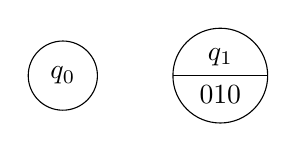
\begin{tikzpicture} [node distance = 2 cm, on grid]
  \node (q0) [state without output] {$q_{0}$};
  \node (q1) [state with output, right = of q0] {
    $q_{1}$ \nodepart{lower} $010$
  };
\end{tikzpicture}
\end{document}
